\chapter{GETTING STARTED WITH \MakeUppercase{\appName} TOOL}
This chapter describes how to create an analysis report using \appName\ and save analyzed result for future use. This chapter contains the following topics:
\begin{itemize}
  \item Running \appName
  \item Making connection and loading ECM systems
  \item Overview of \appName\ window Settings for \appName
  \item Generating Report
  \item Analyzing the report generated
  \item Saving and loading, exporting the analyzed report
  \item Features of Analyzer
\end{itemize}
 \section{RUNNING \MakeUppercase{\appName} REPORT}

\subsection{Running \appName}
\begin{itemize}
\item[--] To run \appName, click Start > All Programs > Tzunami > \appName\ - for windows 7 or older version, or
For windows 10 and above
Click    button and scroll through the alphabetical list for Tzunami. Under this locate \appName\ and click it to run. ECM Selection wizard appears as follows:
\begin{figure} 
  \centering
	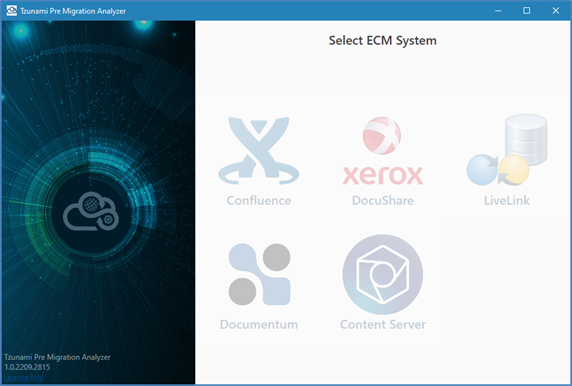
\includegraphics[width=0.8\textwidth]{Images/SelectEccmScreen.png}
 \caption{Select ECM System screen}
\end{figure}
\item[--] Next select the required ECM system for the Analysis of the source content.
\end{itemize}
\section{MAKING CONNECTION AND LOADING ECM SYSTEMS}
\subsection{Making connection with the ECM system}
Run \appName\ Tool. The home screen appears as mentioned above. Now, click the icon of the required ECM system. Respective connection wizard will pop up for the respective ECM system. Provide necessary information to connect with the ECM system and proceed further.\\
According to the supported ECM type making connection with them is explained below:
\subsection*{Making connection with Confluence Server:}
To make the connection with Confluence Server using \appName, the first thing to check is whether the Remote APIs are enabled in the Confluence Administration Console or not. If not, please follow the instruction given below, and the setting for all versions of confluence is the same.\\
Steps to enable Remote API:
\begin{enumerate}
	\item Go to the Confluence 'Administration Console':
	\begin{itemize}
		\item Choose Browse > Confluence Admin. The 'Administrator Access' login screen will be displayed.
		\item Enter your password and click Confirm. You will be temporarily logged into a secure session to access the 'Administration Console'.		
	\end{itemize}
	\item Select 'General Configuration' in the left-hand panel.
	\item Click 'Edit' next to ‘Feature Settings’.
	\item To enable Remote API, check 'Remote API (XML-RPC \& SOAP)'
	\item Click 'Save' to retain the changes made.
\end{enumerate}
	Also, the user account used for making connection with Confluence Server should have following permissions:
	\begin{itemize}
		\item User must be member of confluence-administrator Groups.
		\item User must be a member of confluence-user group.
	\end{itemize}
Another thing to keep in mind is proxy settings, this must be disabled to avoid conflict between \appName\ and Confluence server. For more information, please contact your system administrator.
\subsection*{To make connection with Confluence Server:}
\begin{enumerate}
	\item Click the Confluence Server icon, connection screen appears as follows:
	\begin{figure} 
		\centering
		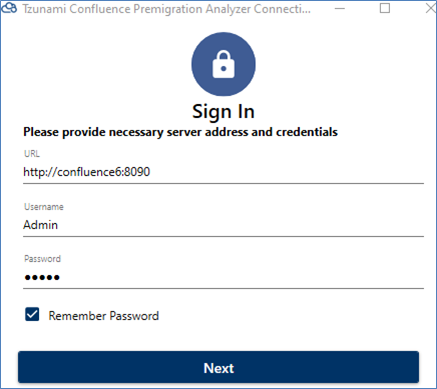
\includegraphics[width=0.8\textwidth]{Images/Confluence connection wizard.png}
		\caption{Confluence connection wizard}
	\end{figure}
\item Provide the required portal credential to connect to the Confluence server as instructed in table given below:
\begin{table*}[] \centering
	%\ra{1.3}
	\begin{small}
		\begin{tabular}{@{}lrrrrrrrrrrrr@{}} \toprule
			\textbf{Field}  & \textbf{Description} \\ \midrule 
			\textbf{URL} & Enter the URL of the Confluence Server.\\ 
			\textbf{Username} & Enter the username to use when connecting to Confluence Server.\\ 
			\textbf{Password} & Enter the password of the user.\\ [1ex]
			\bottomrule
		\end{tabular}
	\end{small}
	\caption{Connection Description Fields for Confluence}
	\label{table:Confluence} % is used to refer this table in the text
\end{table*}
\item Click Next Button.
\end{enumerate}
\subsection*{To make connection with DocuShare Server:}
To analyze the content of DocuShare Server, the Analyzer must be allowed to connect with the database server. The tool supports two types of data base provider. They are:
\begin{enumerate}
	\item Microsoft SQL server
	\begin{figure} 
		\centering
		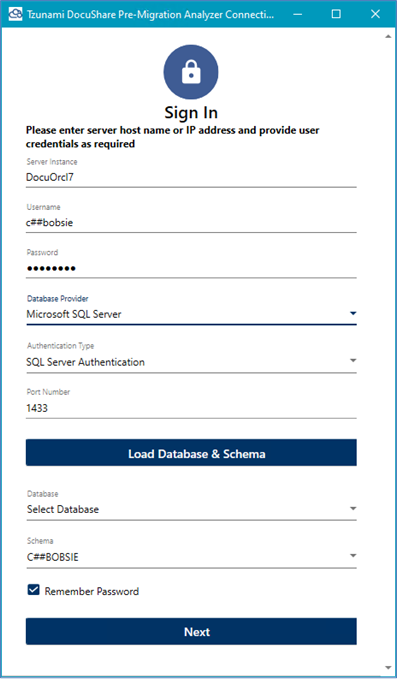
\includegraphics[width=0.8\textwidth]{Images/DsConnectonMsSql.png}
		\caption{Connection wizard for DocuShare (Microsoft SQL Server)}
	\end{figure}\\
{In order to make the database connection with Microsoft SQL server type, fill in the parameters given in the table below:}
	\end{enumerate}
